% 1. [dvipdfmx] をここに書く
\documentclass[dvipdfmx,a4paper,10.5pt]{jarticle}

% --- 数式関連 ---
\usepackage{amsmath, amsfonts, amssymb}
\usepackage{bm}
\usepackage{mathtools}
\usepackage{empheq}

% --- 図・色・レイアウト ---
\usepackage{graphicx}
\usepackage{xcolor}
\usepackage{float}
\usepackage{fancyhdr}
\usepackage{siunitx}
\usepackage{longtable}
\usepackage{booktabs}
\usepackage[most]{tcolorbox}

% --- TikZ関連 ---
\usepackage{tikz}
\usepackage{tikz-3dplot}
\usetikzlibrary{positioning, arrows.meta, shapes.geometric, calc, decorations.pathreplacing, decorations.markings, patterns}
\usepackage{pgfplots}
\usepgfplotslibrary{statistics} % boxplotに必須
\pgfplotsset{compat=1.18}

% --- その他 ---
\usepackage{listings,jvlisting}
\usepackage{otf}
\usepackage{ascmac}
\usepackage[margin=20mm]{geometry}

% --- ハイパーリンク ---
\usepackage[
  dvipdfmx,
  colorlinks=true,
  linkcolor=black,
  citecolor=black,
  urlcolor=black
]{hyperref}
\urlstyle{same}

\newcommand{\marker}[2]{%
  \text{%
    \begingroup
    \setlength{\fboxsep}{1.5pt}%
    \colorbox{#1!20}{$\displaystyle #2$}%
    \endgroup
  }%
}

\lstset{
    language=Python,
    basicstyle=\ttfamily\small,
    keywordstyle=\color{blue},
    commentstyle=\color{gray},
    stringstyle=\color{red},
    numbers=left,
    numberstyle=\tiny\color{gray},
    breaklines=true,
    frame=single,
    showstringspaces=false,
    showspaces=false,
    showtabs=false,
}

\newcommand{\prob}[1]{\section*{\,\bm{\fbox{#1}}\,}}
\numberwithin{equation}{section}

% --- レジュメ用 ---
% 要点をまとめる枠
\newtcolorbox{point}[1][]{colback=blue!3, colframe=blue!50!black, boxrule=0.6pt, arc=2pt, fonttitle=\bfseries, #1}
% 講義スライドの切り出し（上段・下段のスライド）
\newcommand{\slidetop}[3]{\includegraphics[page=#2,trim=32 383 31 70,clip,width=#3]{figs/#1.pdf}}
\newcommand{\slidebot}[3]{\includegraphics[page=#2,trim=32 70 31 383,clip,width=#3]{figs/#1.pdf}}
\newcommand{\pd}[2]{\frac{\partial #1}{\partial #2}}
\newcommand{\Pd}[2]{\frac{\partial^2 #1}{\partial #2^2}}
\newcommand{\DDt}{\frac{D}{Dt}}
\renewcommand{\div}{\operatorname{div}}
\newcommand{\grad}{\operatorname{grad}}
\newcommand{\rot}{\operatorname{rot}}

\newcommand{\cov}{\operatorname{cov}}
\newcommand{\Var}{\operatorname{var}}

\title{今週のまとめ：EnKC の修正量の式から見た制御の実験}
\author{}
\date{2026年11月4日}
\setlength{\headheight}{15pt}
\addtolength{\topmargin}{-3pt}
\pagestyle{fancy}
\lhead{}
\rhead{}

\begin{document}
\maketitle
\tableofcontents
\clearpage

%======================================================================
\section{話の軸：修正量の式}
%======================================================================

目標 $Y$（目標領域 20\,km 四方の 13〜17 時の雨の合計）が 1 つのとき，EnKC が土壌水分 $\theta$ に足す修正量は
\begin{equation}
  \boxed{\;\Delta\theta=\frac{\cov(\theta,Y)}{\Var(Y)+\sigma_R^2}\,\bigl(y^*-\bar Y\bigr)\;}
  \label{eq:dtheta}
\end{equation}
である．意味は「\textbf{雨が目標 $y^*$ に近かった member の土壌水分の側へ，真値の土壌水分を寄せる}」．

\begin{center}
\begin{tabular}{lp{0.5\textwidth}l}\toprule
項 & 意味 & 今週の値 \\ \midrule
$\cov(\theta,Y)$ & 雨の少なかった member と多かった member で，土壌水分がどう違ったか & ほぼ 0（\S\ref{sec:1}，\S\ref{sec:2}） \\
$\Var(Y)+\sigma_R^2$ & 雨のばらつき．$\sigma_R=\sigma_Y$ なので差の半分を詰めにいく & $2\times3.9^2$\,mm$^2$ \\
$y^*-\bar Y$ & 目標とアンサンブル平均の差 & $8-8.95=-0.95$\,mm \\ \bottomrule
\end{tabular}
\end{center}

うまくいくための前提は 2 つある．
\begin{enumerate}
  \item \textbf{cov が大きい}：雨の少なかった member は，土壌水分が違ったから雨が少なかった
  \item \textbf{足せばそのとおりに動く}：真値に $\Delta\theta$ を足すと，雨は $\cov(\theta,Y)/\Var(\theta)\times\Delta\theta$ だけ動く（線形）
\end{enumerate}
今週の結果は，\textbf{この 2 つがどちらも成り立たなかった}，とまとめられる．

%======================================================================
\section{制御実験の条件}\label{sec:cond}
%======================================================================

\subsection{系と役割}
\begin{center}
\begin{tabular}{p{0.2\textwidth}p{0.68\textwidth}}\toprule
モデル & SCALE-RM，水平 2\,km，$120\times120$ 格子（240\,km 四方），二重周期，全面陸，バケツ型の土壌（7 層），日射は固定（日変化なし） \\
真値（現実） & mdet．観測は mdet の予報にノイズを足したもの．\textbf{制御はこの mdet に介入する} \\
アンサンブル & Phase 8：80 member，毎時 LETKF で同化（0〜24 時，制御なし）．
              8 時の解析を出発点として，\S\ref{sec:sens} の感度の予報に使う \\ \bottomrule
\end{tabular}
\end{center}

\subsection{目標}
\begin{center}
\begin{tabular}{p{0.2\textwidth}p{0.68\textwidth}}\toprule
場所 & x 70〜90\,km・y 110〜130\,km の 20\,km 四方（$10\times10$ 格子）．Phase 8 の mdet で 12〜24 時の積算がいちばん多い 20\,km 格子 \\
目標の量 $Y$ & 目標領域で平均した雨の，\textbf{13〜17 時の合計}（決定）．比較のため 13〜14 時の雨（降り始め）も試した \\
目標値 $y^*$ & 13〜17 時：8\,mm（決定）．13〜14 時：0\,mm（仮に置いた値） \\
目標の誤差 $\sigma_R$ & $\sigma_R=\sigma_Y$（80 member の $Y$ の標準偏差）．差の半分を詰めにいく \\ \bottomrule
\end{tabular}
\end{center}

\subsection{介入}
\begin{center}
\begin{tabular}{p{0.2\textwidth}p{0.68\textwidth}}\toprule
修正する変数 & 土壌水分の第 1・2 層（0〜20\,cm）．両層に同じ $\Delta\theta$ を足し，0〜0.5 に切り詰める \\
時刻・回数 & 8 時に 1 回．13 時の降り始めまで 5 時間 \\
向き & 増やす向きだけ（$\Delta\theta<0$ を 0 にする，「clip」）．比べるため，切らない場合（「noclip」）も流した \\
範囲（状態の表し方） & full：全格子で式 \eqref{eq:dtheta} をそのまま使う．\\
 & local：目標のパッチと周りの 8 パッチ（$3\times3$ パッチ）の平均の 2 自由度に絞り，それぞれ一様に足す．外は 0 \\ \bottomrule
\end{tabular}
\end{center}

\subsection{感度（cov）を見積もるアンサンブル}\label{sec:sens}
\begin{itemize}
  \item Phase 8 の 8 時の解析（80 member）に，20\,km 四方のパッチごとの一様乱数の土壌水分の摂動
        （標準偏差 0.02，第 1・2 層，目標領域がちょうど 1 パッチ）を足し，\textbf{同化なしで 18 時まで予報}した．mdet には足さない
  \item 式 \eqref{eq:dtheta} の $\theta$ の member の違いは，この摂動で表す（8 時の解析そのもののばらつき 約 0.001 は無視）
  \item $\cov(\theta,Y)$，$\Var(Y)$，$\bar Y$ はすべて，この 80 member を標本として計算した
\end{itemize}

\subsection{比べたもの（11 本．いずれも mdet の 8 時から 18 時まで予報）}
\begin{center}
\begin{tabular}{lll}\toprule
本 & 目標 & 修正 \\ \midrule
修正なし & --- & なし（流し直し．もとの mdet とビット単位で一致） \\
EnKC 4 本 $\times$ 2 目標 & 13〜14 時 / 13〜17 時 & full・local $\times$ clip・noclip \\
ランダム 1 本 $\times$ 2 目標 & 13〜14 時 / 13〜17 時 & local・clip の修正を，離れた場所へずらす \\ \bottomrule
\end{tabular}
\end{center}
評価は，目標領域の 13〜14 時の雨，13〜17 時の合計，降り始めの時刻（目標領域の平均が 1\,mm/h を超えた時刻）．
修正なしの mdet の 13〜17 時の合計は 8.06\,mm（Phase 8 の cycle の中の mdet は 12.6\,mm．
8 時から 1 本で流すと 9 時まではビット単位で一致し，その後カオスで離れる）．

%======================================================================
\section{Phase 8 のアンサンブル：土壌水分のばらつきがない}\label{sec:1}
%======================================================================

\begin{itemize}
  \item 初期（0 時）に入れた土壌水分の摂動（$\pm0.01$，2\,km の白色雑音，表層のみ）は，8 時には標準偏差 約 0.001 まで薄まった
  \item $\cov(\theta,Y)=\rho\,\sigma_\theta\sigma_Y$ の $\sigma_\theta$ がほぼ 0 なので，\textbf{cov もほぼ 0}．格子ごとの相関も，0〜12 時のどの時刻でも偶然と区別できない
  \item 式 \eqref{eq:dtheta} の修正量はほぼ 0 で，そもそも制御が始まらない
\end{itemize}

%======================================================================
\section{8 時にばらつきを入れ直しても：雨は土壌水分で決まっていない}\label{sec:2}
%======================================================================

8 時に 20\,km 四方のパッチごとの摂動（標準偏差 0.02，0〜20\,cm）を入れて，80 member を 18 時まで予報した．

\begin{itemize}
  \item 土壌水分 $\to$ Bowen 比はほぼ決定的（相関 $-0.99$）．地表と境界層は土壌水分どおりに動く
  \item 雨は動かない．目標のパッチの摂動と 13〜17 時の合計の相関は $-0.17$（偶然と区別できない）．
        降り始め（13〜14 時の雨）とは $-0.66$ で，湿らせると降り始めが遅れる
  \item \textbf{雨のばらつきは，摂動を入れてもほとんど増えない}：13〜17 時の合計は Phase 8 で $8.75\pm3.54$\,mm，パッチの摂動ありで $8.95\pm3.90$\,mm
\end{itemize}
つまり member の雨の違いは，ほとんどが\textbf{大気の違い（8 時の解析の違いと，その後のカオス）}から来ている．
雨の少なかった member は，土壌水分のおかげで少なかったわけではない．だから cov が小さい（前提 1 が成り立たない）．

数字を入れると，式 \eqref{eq:dtheta} の修正量は
\begin{equation}
  \Delta\theta=\underbrace{-0.17}_{\rho}\times\frac{\overbrace{0.0197}^{\sigma_\theta}}{\underbrace{3.93}_{\sigma_Y}}\times\underbrace{0.5}_{\sigma_R=\sigma_Y}\times\underbrace{(-0.95)}_{y^*-\bar Y}\approx+0.0004
\end{equation}
で，ばらつき（0.02）の 50 分の 1 しかない．予測される雨の変化は $-0.01$\,mm．

%======================================================================
\section{それでも足してみた：効果は見えない}\label{sec:3}
%======================================================================

この修正量を真値（mdet）の 8 時の土壌水分に足し，18 時まで流した（11 本，約 5 分）．
比べるために，同じ修正をランダムな場所に足した本も流した．

\begin{figure}[H]
\centering
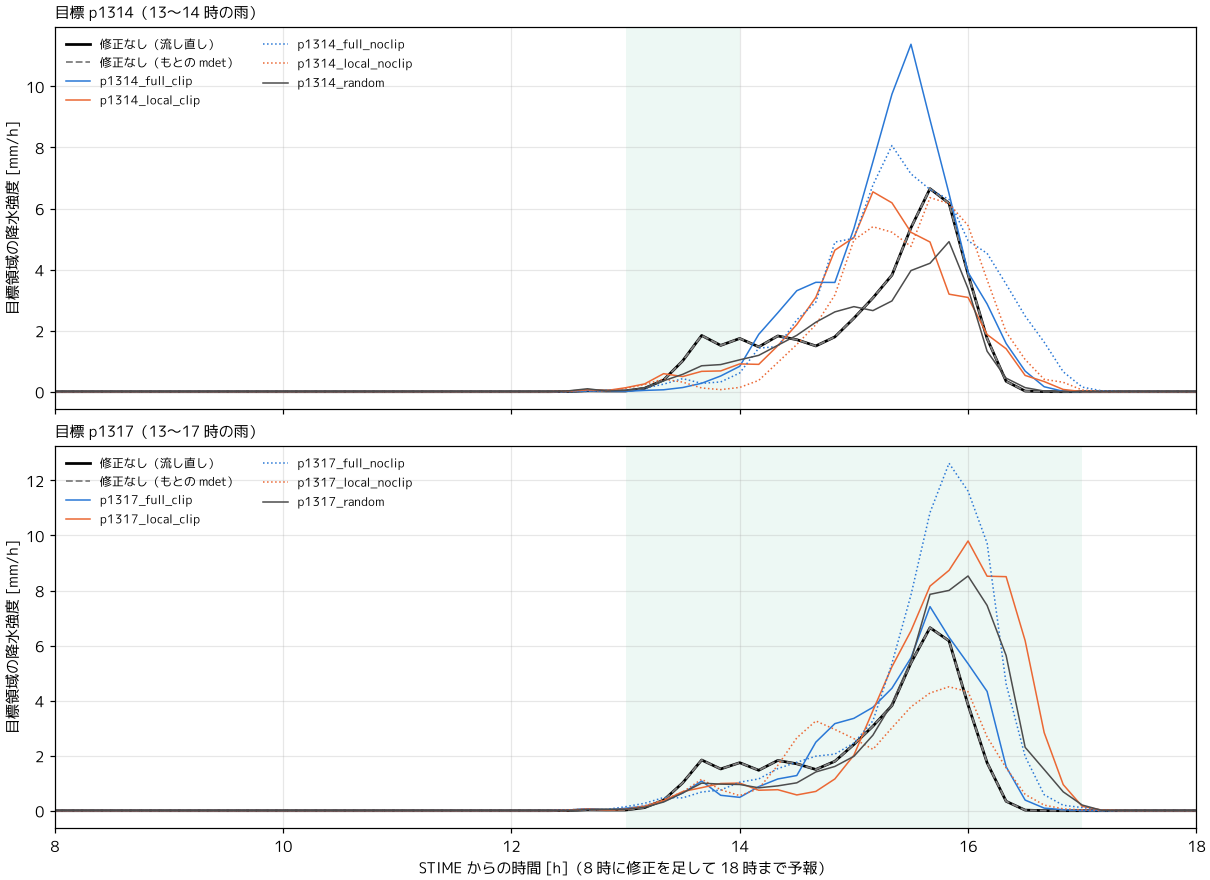
\includegraphics[width=\textwidth]{../20261103_enkc_once/control_target.png}
\caption{目標領域の降水強度．黒：修正なし．色：EnKC の修正あり（full / local，湿らせるだけ / 切らない）．灰色の実線：ランダムな場所に足した本．}
\label{fig:control}
\end{figure}

\begin{itemize}
  \item 修正なしで流し直した本は，もとの mdet とビット単位で一致した（差は修正だけによる）
  \item 修正（0.0004〜0.006）を足すと，13〜17 時の合計は 10 本で平均 $+2.4$\,mm，標準偏差 2.5\,mm 変わった．
        予測（$-0.01$〜$-0.06$\,mm）より 2 桁大きく，向きもばらばら
  \item \textbf{ランダムな場所に足した本も，同じくらい変わった}
\end{itemize}
どんな小さな修正でも，5 時間のうちにカオスで育ち，雨は別の道に乗り換わる（前提 2 が成り立たない）．
式 \eqref{eq:dtheta} の効果は，この揺れに埋もれて検出できない．

%======================================================================
\section{目標を Bowen 比などに替えたら？}
%======================================================================

Bowen 比なら $\rho\approx-0.99$ で，cov が大きく，修正量は $y^*$ の置き方しだいでばらつき程度まで出せる．
しかし Bowen 比・境界層の高さ・LCL は土壌水分でほぼ決まる量で，雨について土壌水分以上の情報を持たない
（土壌水分の影響を除くと，降り始めとの相関は $|r|\le0.2$）．
雨が動く量は，結局「土壌水分 $\to$ 雨」の効き方で決まり，\S\ref{sec:2} と同じになる．
代わりの目標は，土壌水分で動かせて，かつ雨の仕組みに近い情報を持つ量である必要がある（候補は相談したい）．

%======================================================================
\section{今週の報告}
%======================================================================

\begin{point}[title=報告すること]
\begin{enumerate}
  \item \textbf{Phase 8 のアンサンブルでは，土壌水分のばらつきが小さくなっていた}（8 時に約 0.001）．
        式 \eqref{eq:dtheta} の cov がほぼ 0 で，EnKC は効き方を学べない
  \item \textbf{8 時にばらつきを入れ直しても，EnKC ではうまくいかなかった}．
        雨のばらつきは大気の違いとカオスで決まっていて，土壌水分との cov が小さい．
        修正量は 0.0004 にとどまり，真値に足しても，その効果は修正を入れただけで起きるカオスの揺れ（約 2.5\,mm）に埋もれた
  \item \textbf{代わりの物理量を考えたい}．Bowen 比・PBL・LCL は土壌水分の写しで，それだけでは足りない
\end{enumerate}
\end{point}

\paragraph{台風（Sawada et al.\ 2026）との違い}
台風では，良い道を決めている大気の量（最下層の水蒸気）を直接動かし，1 時間先を見て毎時押し直していた．
今回は，間接的な量（土壌水分）を，5 時間先を見て 1 回だけ押している．
次の方向（相談したい）：大気の量も制御する変数に入れる / 雨に近い時刻で短いホライズンの介入を繰り返す /
効果を 1 本の結果でなく分布のずれで評価する．

\end{document}
